% 2005 年湖北卷文科第 20 题配图：长方体被截面 AEC_1F 截得的多面体
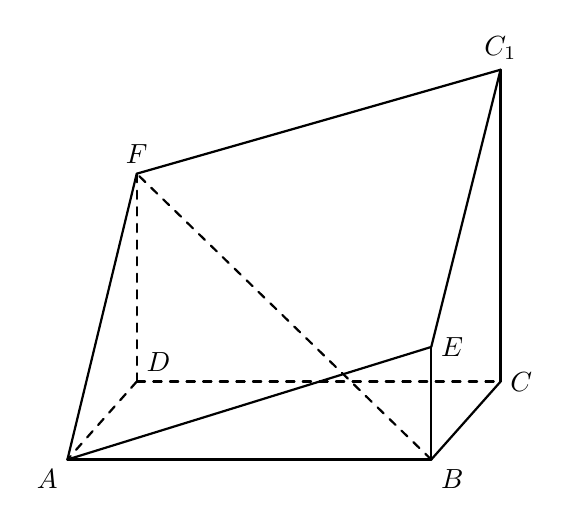
\begin{tikzpicture}[>=stealth,scale=1.1,line cap=round,line join=round]
  % 顶点坐标设定
  \coordinate (D) at (0,0);
  \coordinate (C) at (4.2,0);
  \coordinate (A) at (-0.8,-0.9);
  \coordinate (B) at (3.4,-0.9);
  \coordinate (C1) at (4.2,3.6);
  \coordinate (E) at (3.4,0.4);
  \coordinate (F) at (0,2.4);

  % 虚线不可见棱及内部辅助线
  \draw[dashed,thick] (D) -- (A);
  \draw[dashed,thick] (D) -- (C);
  \draw[dashed,thick] (D) -- (F);
  \draw[dashed,thick] (B) -- (F);

  % 实线可见棱及截面边界
  \draw[thick] (A) -- (B);
  \draw[thick] (B) -- (C);
  \draw[thick] (C) -- (C1);
  \draw[thick] (B) -- (E);
  \draw[thick] (A) -- (E);
  \draw[thick] (E) -- (C1);
  \draw[thick] (C1) -- (F);
  \draw[thick] (F) -- (A);

  % 顶点标签
  \node[below left] at (A) {$A$};
  \node[below right] at (B) {$B$};
  \node[right] at (C) {$C$};
  \node[above right] at (D) {$D$};
  \node[above] at (C1) {$C_1$};
  \node[right] at (E) {$E$};
  \node[above] at (F) {$F$};
\end{tikzpicture}
